%!TEX root = ../PhDthesis.tex
\chapter{Exploring the role of inhibition in cortical development and surround modulation}

Surround suppression is one of the most well described phenomena in
neural circuits, yet no definite conclusions on the sources of various
forms of suppressions can be drawn so far. In the literature section
of this thesis we described the known properties of various inhibitory
cell classes and what roles they might perform. In particular we
discovered that PV and SOM-expressing interneurons exhibit highly
distinct response properties and layer-specific expression patterns.
With recent techniques allowing targeting of specific populations
there is now huge interest in understanding their role both in
development and in mediating and gating the both contextual and
attentional modulation phenomena.

In this chapter we will propose models that incorporate the distinct
response properties of PV and SOM interneuron populations, allowing us
to make concrete predictions about their role in developmental and
behavioural phenomena. First we establish that the fast response and
linear response of the PV-ir, fast-spiking interneuron population
makes them ideally suited towards controlling feedforward activity,
sparsifying activity and thereby driving map formation. While
demonstrating robust and stable map formation even in the presence of
strong lateral excitation, we show that the broad tuning properties of
the PV population makes them badly suited to mediate context and
feature specific modulation. By introducing a secondary inhibitory
population modeled on the response properties of SOM+ neurons we
extend the model to demonstrate how their weaker and facilitating
inputs \citep{Bartley2008,Beierlein2003,Bartley2008,Tan2008} lead to
the development of highly tuned neurons, which respond only for high
contrasts or large stimuli, thereby mediating a range of surround
modulation phenomena.

\section{Methods}

\subsection{Assessing the quality of orientation maps}

In addition to assessing the spatial scales in the model and comparing
them against experiment the model developed in this section should
also share other properties including robustness to a variety of
visual input, as well as smooth, robust and high-quality organization
of V1 neurons into an overall orientation map. There are a variety of
measures to assess these properties but we will focus on three in
particular, smoothness, stability and pinwheel density.

\subsubsection{Pinwheel density}

Through empirical observation that orientation maps across species
share a fundamental property, that pinwheel count in biological
orientation maps scales linearly with hypercolumn size, specifically
that there are $\pi$ orientation pinwheels within the area of one
hypercolumn, when averaging over sufficiently large cortical
areas. This dimensionless, statistical measure of pinwheel
distribution is thought to reflect a universal constant of map
organization, converging to across carnivorans, primates, cats, and
tree shrews \citep{Kaschube2010, Keil2012}. This value was predicted
by a theoretical model of map organization and has strong empirical
evidence, with a mean pinwheel density across four species (tree
shrew, galago, cat, and ferret) statistically indistinguishable from
$\pi$.

To determine the pinwheel density for any given map, the hypercolumn
distance is computed and all all pinwheel centers are found. Pinwheel
centers are located at the intersection of the zero contours of the
real and imaginary components in the polar representation of
orientation preference \citep{Lowel1998}. Then we simply divide the
number of pinwheels in the modelled area by the number of hypercolumns
to arrive at the pinwheel density.

\subsubsection{Stability}

The stability of orientation maps is determined by determing the
average orientation similarity index of the orientation map over the
course of development. To assess similarity quantitatively
\cite{Chapman1996} computed the correlation of orientation preference
at each developmental age with the organized preference map observed
in the final recording for that animal. As in \cite{Stevens2013} we
normalize these similarity values to fall between 0 (completely
uncorrelated) to 1 (identical orientation preference). The orientation
similarity index is therefore defined as:

\begin{equation}
  OSI = 1 - \frac{4}{n\pi} \sum_{i}\abs{(F_{i}-O_{i})mod(\frac{\pi}{2})}
\end{equation}

By averaging the OSI at every 1000 development steps we can
numerically compare the stability of the model over time. Note that
this does not provide a measure that is comparable across models
because this measure is heavily influenced by the speed of learning
but it does allow us to assess the effect of changing specific
parameters on the stability of the model.

\subsection{Surround modulation}

Beyond measuring simple attributes of the spatial organization in LGN
and V1, higher order effecs can be explored through complex surround
modulation measurement protocols. In addition to the simple area
summation curve measurements described above we replicate two further
protocols to evaluate the spatial response properties of the model.
In particular we are interested in the interaction between the spatial
arrangement of visual patterns presented to an animal and the contrast
on the response properties of visually responding neurons. For that
purpose we replicate two measurement protocols, a simple annulus based
contrast suppression measurement \cite{Jones2002} and a protocol using
target and flanker stimuli performed by \cite{Kapadia1995}.

\paragraph{Orientation contrast suppression}

The orientation contrast suppression is perhaps one of the most well
studied surround modulation paradigms. The measurement involves
presenting stimuli of a central sine grating, optimized to the
preferred size, frequency and orientation of the neuron being
measured. Once the baseline activity has been measured an additional
surround anulus with the same frequency is added and varied in
contrast, size and orientation to measure orientation dependent
interactions between center and surround (as shown in Figure
\ref{ORC_Stimulus}).

\begin{figure}
	\centering
        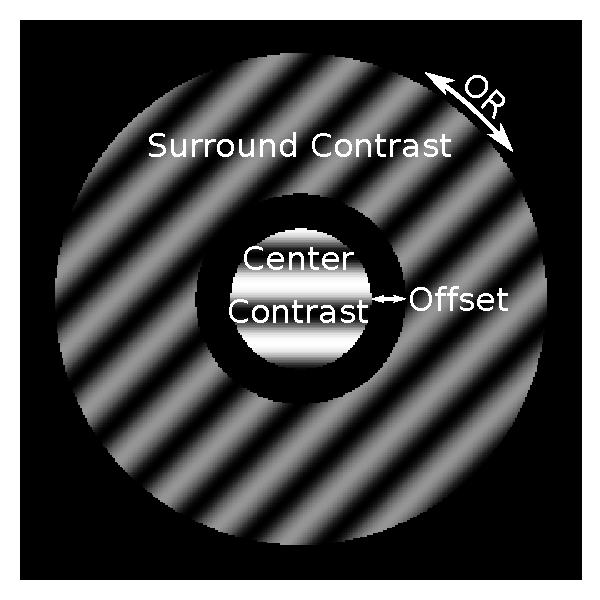
\includegraphics[width=0.5\textwidth]{ORC_Stimulus.pdf}
	\caption{Orientation contrast stimulus measuring modulation by a
      sine grating annulus on the response of a central neuron
      responding to a central sine grating disk of the same frequency.
      Stimulus is varied by center and surround contrast, surround
      orientation and the offset between the central disk and the
      surround annulus.}
	\label{ORC_Stimulus}
\end{figure}

The surround facilitation is quantified as:

\begin{equation}
F = (\frac{R_{cs}}{R_c} - 1) * 100
\end{equation}

where $R_{CS}$ is the response of the combined stimulus and $R_C$ the
response to just the center stimulus.

\paragraph{Flanker Modulation}

Instead of working solely using area based protocols we also make use
of a simple bar based stimulus along with a flanker, which is
modulated in a number of ways to characterize the surround modulation
effects associated with this protocol. In \cite{Kapadia1995} describe
a high degree of variability ranging from a complete lack of surround
modulation to facilitation and suppression. The three stimulus
protocols employed here are shown in \ref{Flanker}, we replicate these
protocol on the model to compare the effects observed in experiments
qualitatively.

\begin{figure}
	\centering
        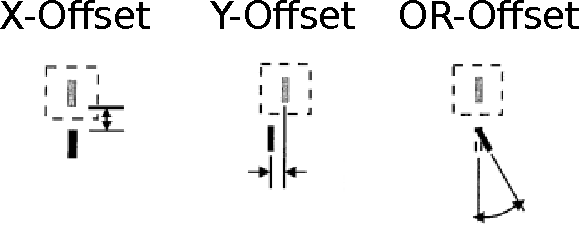
\includegraphics[width=1.0\textwidth]{FlankerProtocol.pdf}
	\caption{Flanker offset surround modulation paradigm. Measuring
      the effect of a flanker stimulus varying by an offset in X, Y
      and orientation on the response of a neuron to a target
      stimulus.}
	\label{Flanker}
\end{figure}


\section{Results}

A major component of the work in this chapter was optimizing for a
wide range of measures to achieve rough agreement with the wide range
of experimentally confirmed measurements. In the coming sections we
will break down how the model parameters were chosen and then compare
measurements and analyses applied to the model to the experimental
results they are replicating, highlighting discrepancies and
simplifications where there are any.

\section{The role of inhibition in development}

Most developmental models of the primary visual cortex are based
around the concept of so called Mexican hat connectivity. This is the
idea that there is a local attractive force which pulls similar
features together and a larger repulsive force, which pushes
dissimilar features away. This is what enables the self-organization
of feature maps, which itself can be explained in terms of
dimensionality reduction, specifically forming a discretized
approximation of the principal surface of the input
\citep{Ritter1992}. In most of these models \citep{Miller1994,
  Miikkulainen2005} these interactions are modeled using point neurons
which provide excitatory and inhibitory input. In the previous chapter
we showed that an adapted version of the GCAL model
\citep{Stevens2013}, which employs divisive inhibition can still
demonstrate robust and stable map development. Here we will extend
this

\subsection{The SEPI Model}


\begin{figure}
	\centering
        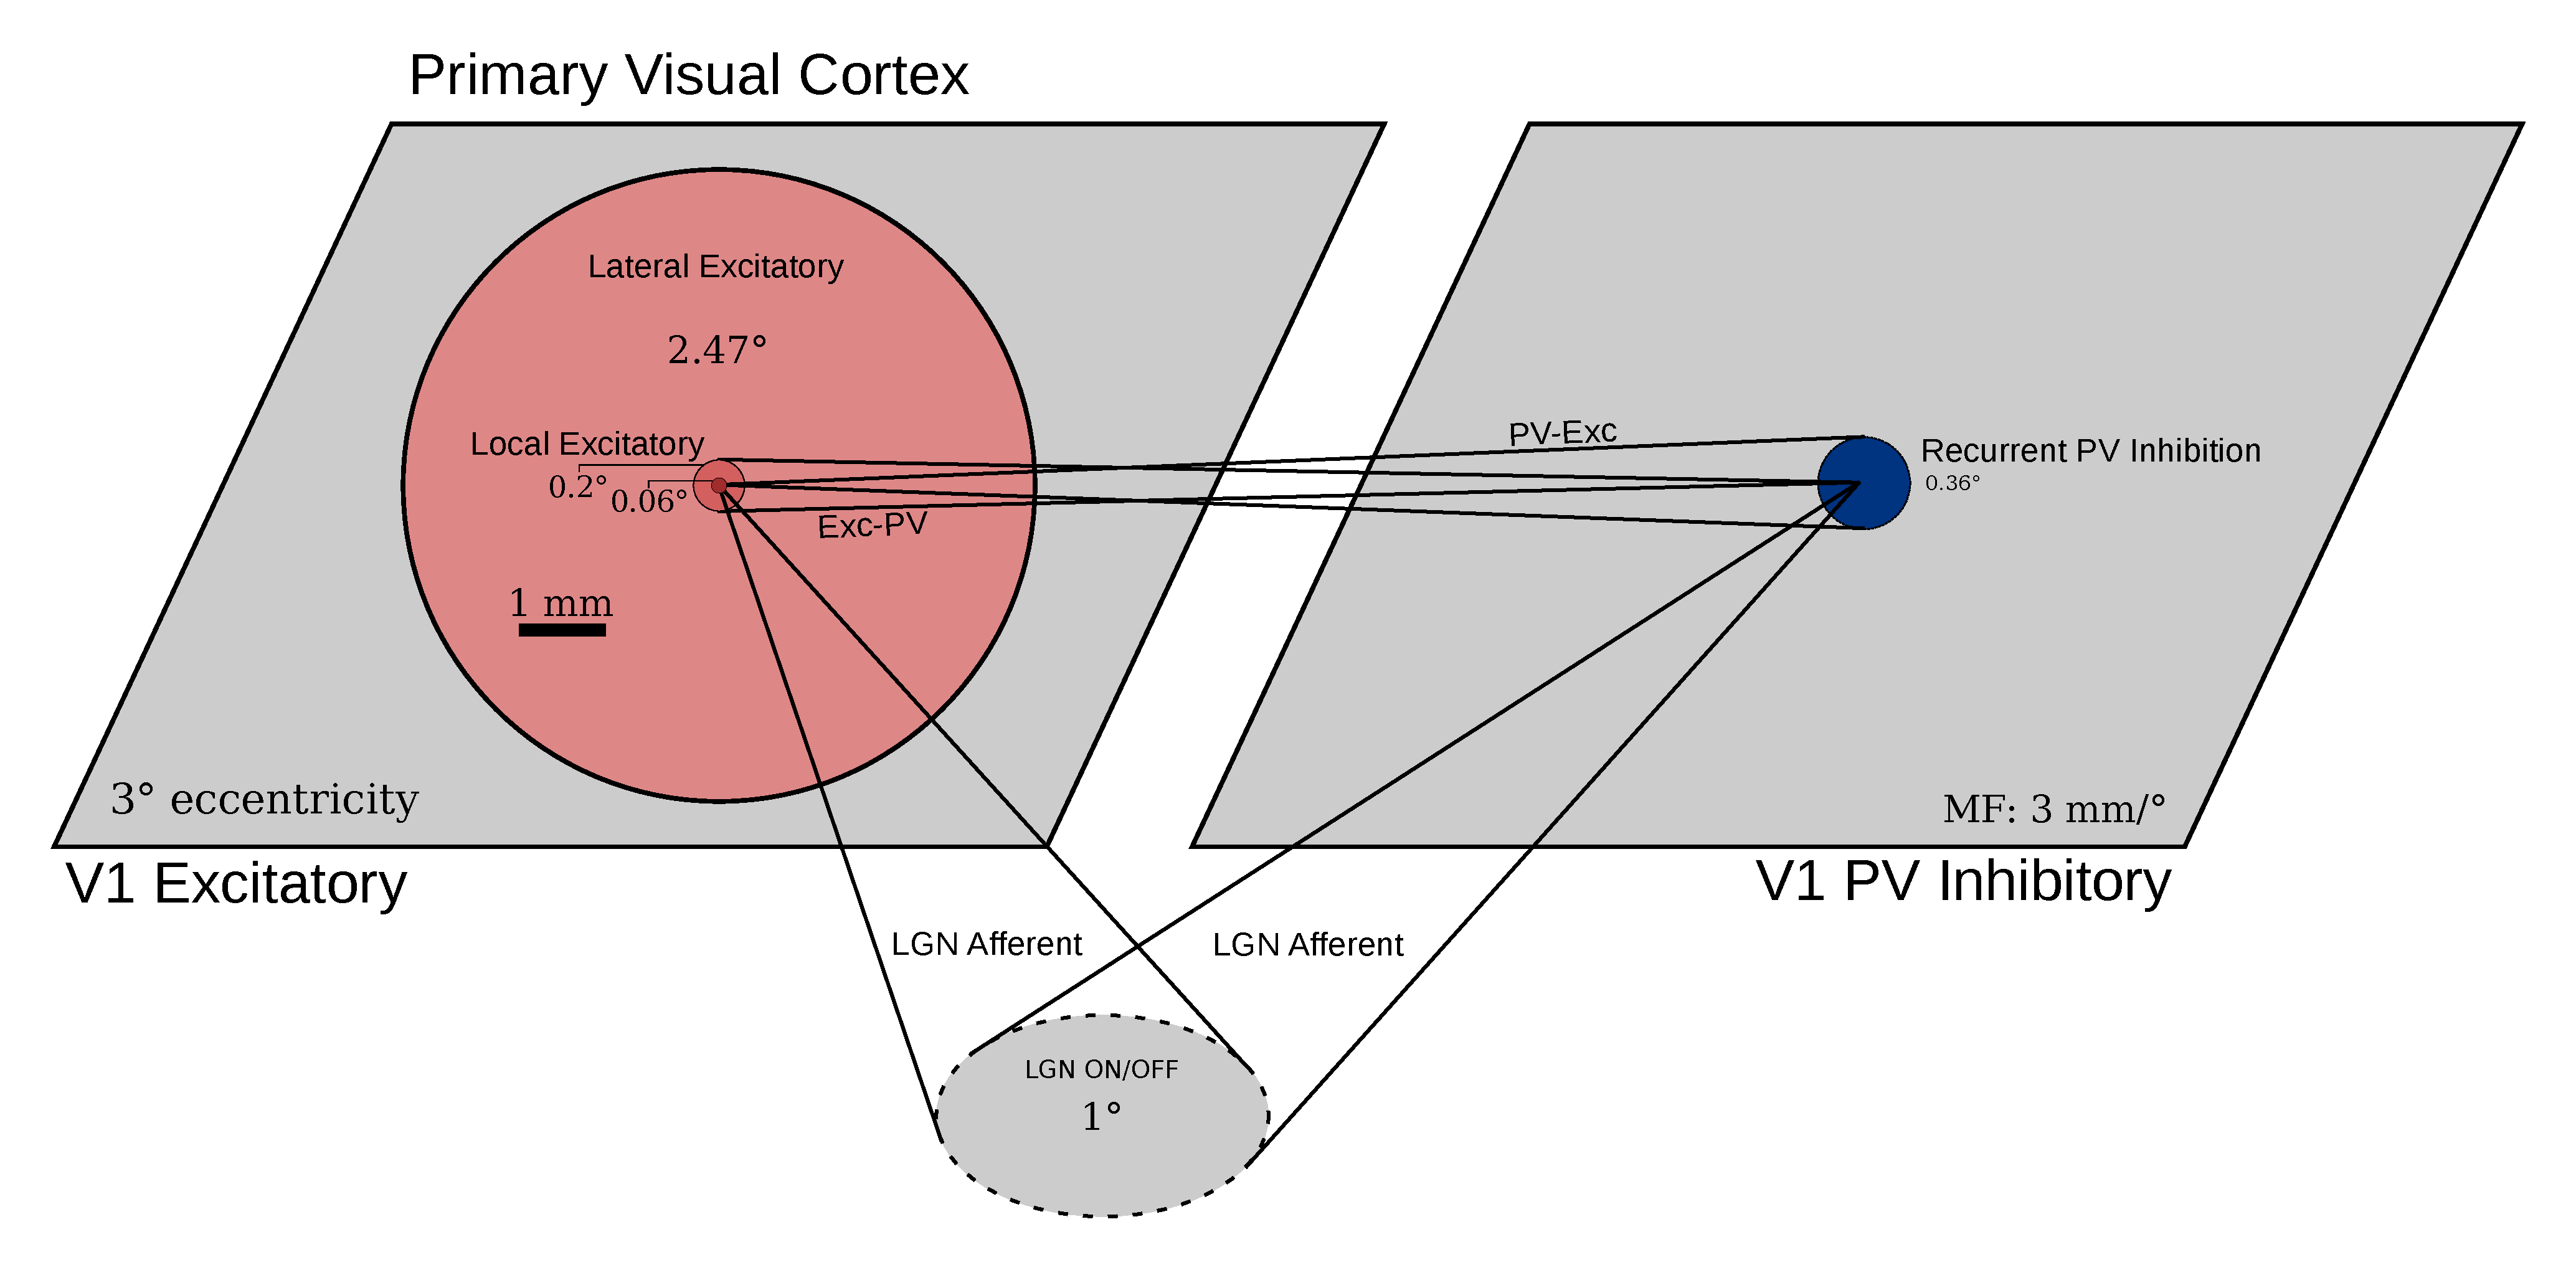
\includegraphics[width=1.0\textwidth]{SEPI_Diagram.pdf}
	\caption{Diagram of the SEPI V1 stage of the model showing the
          spatial scales of the various excitatory (red) and
          inhibitory (blue) connections. Satured colors indicate the
          kernel radii, while lightly shaded regions indicate kernel
          cut-off extents.}
	\label{SCALDiagram}
\end{figure}


\subsection{Results}

\begin{figure}
	\centering
        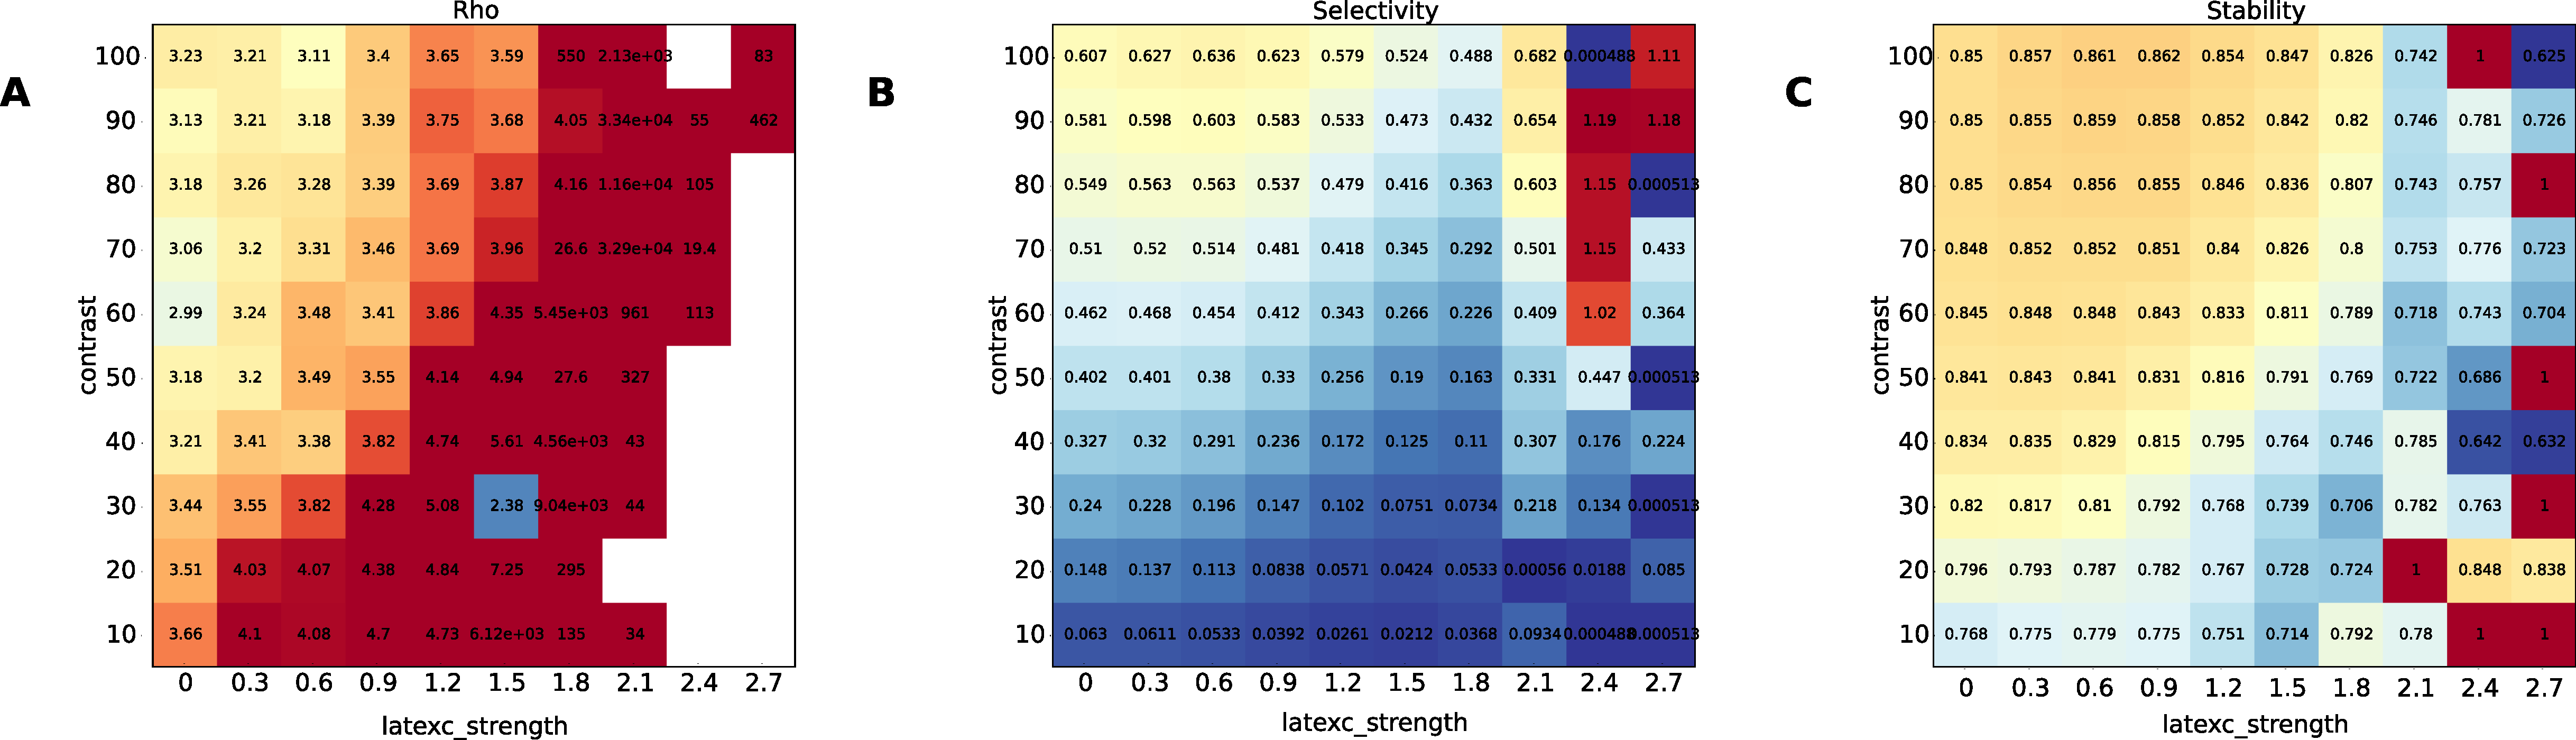
\includegraphics[width=1.0\textwidth]{SCAL_LatStability.pdf}
	\caption{Parameter explorations of three separate metrics of
          orientation map development using the SCAL model. Varied
          parameters are the strength of long-range lateral excitation
          and the stimulus contrast. The three metrics are \textbf{A}
          the $\rho$ pinwheel density metric, which characterizes the
          quality of the map, \textbf{B} the average selectivity over
          the time course of development and \textbf{C} the stability
          metric measuring how much the map changes throughout the
          course of development. The model shows good robustness to
          varying stimulus contrasts at low levels of lateral
          excitation but quickly deteriorates with increasing levels
          of excitation. White values indicate instabilities in the
          model causing the model to terminate.}
	\label{SCALStability}
\end{figure}


\begin{figure}
	\centering
        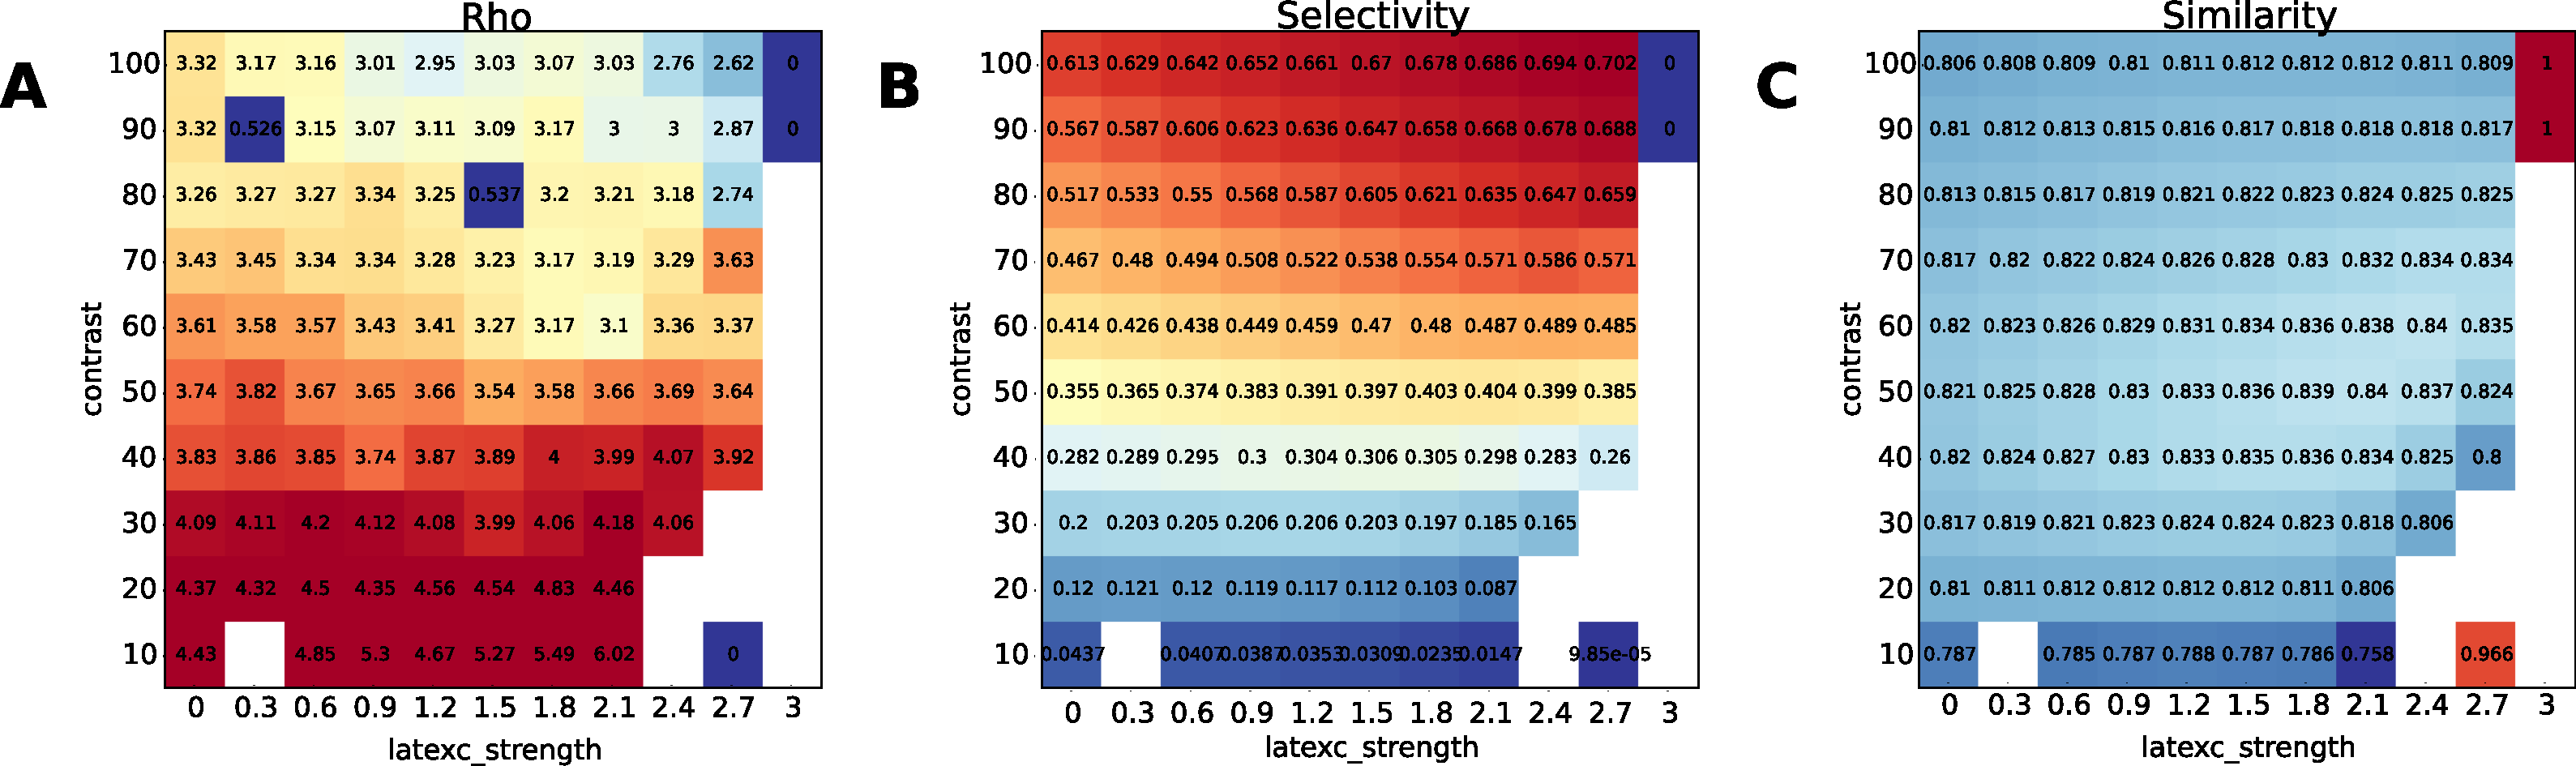
\includegraphics[width=1.0\textwidth]{SEPI_LatStability.pdf}
	\caption{Parameter explorations of three separate metrics of
          orientation map development using the SEPI model. In
          comparison to the SCAL model the pinwheel metric is not as
          robust to changes in contrast, however the model is far more
          robust to strong lateral excitation and maintains almost
          uniform stability across almost all explored parameter
          values. Uncoupling of excitation and inhibition allows the
          model to handle changes in parameter strengths but in
          absence of a homeostatic mechanism may disrupt map formation
          at low contrasts.}
	\label{SEPIStability}
\end{figure}


\section{The role of inhbition in surround modulation}


\subsection{The LESPI model}

\begin{figure}
	\centering
	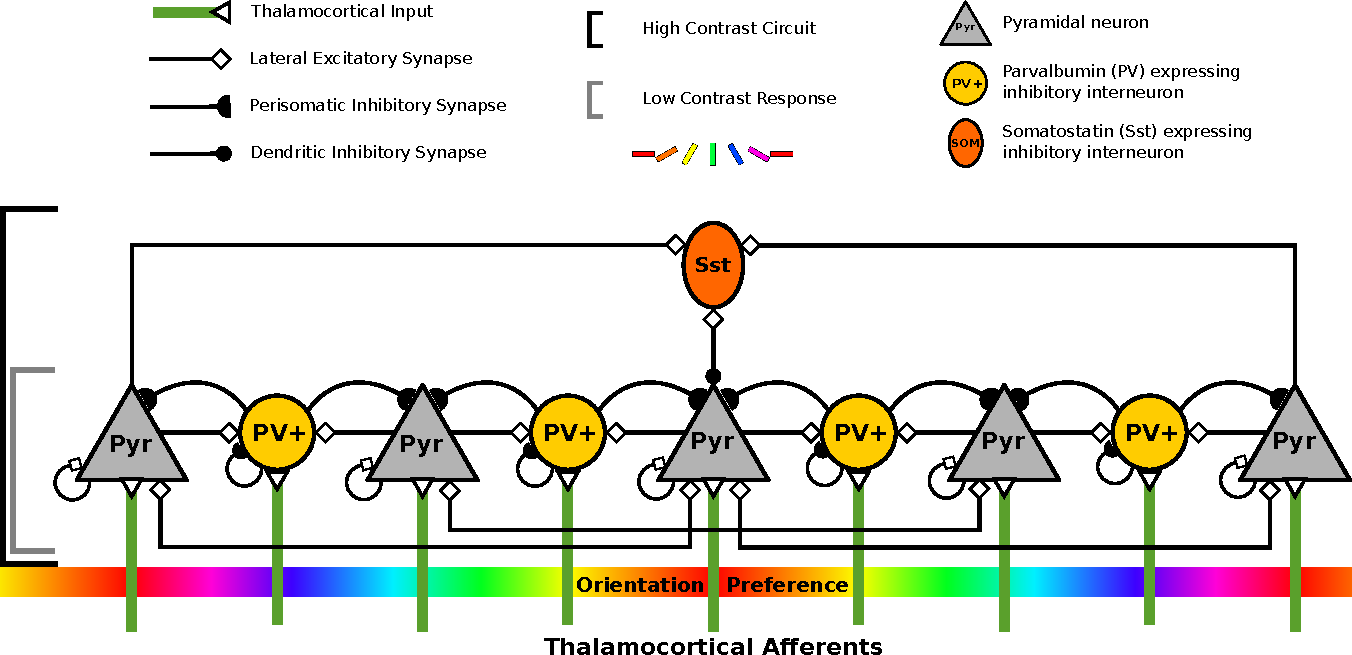
\includegraphics[width=1.0\textwidth]{./v1circuit.pdf}
	\caption[]{High-level circuit diagram of the LESPI model.}
    \label{circuit_diagram}
\end{figure}


\begin{equation}
  \eta_{exc} = \frac{\eta_{A} + \eta_{LOC}}{1 + \eta_{PV}} * \eta_{SM}
\end{equation}

where $\eta_{A}$ is the LGN afferent activity, $\eta_{LOC}$ the local
excitatory contribution, $\eta_{P}$ the PV inhibitory contribution
and the surround modulation term $\eta_{SM}$ is defined as:

\begin{equation}
  \eta_{SM} = 1 + \eta_{LAT} - \eta_{S}
\end{equation}

where $\eta_{LAT}$ represents the long-range lateral excitatory
contribution and $\eta_{S}$ is the Sst inhibitory contribution. In the
SEPI model the $\eta_{SM}$ term simply reduces to 1, eliminating all
long-range interactions. The surround modulatorion term provides gain
when excitation exceeds inhibition and shunting inhibition when the
reverse is true. As such, this term provides a convenient abstraction
to model the modulatory influence of the dendritic integration of
long-range inputs.

The effective excitatory gain may not be a bad approximation to the
effect of long-range horizontal connections, which have been shown to
be strongly voltage dependent \citep{Hirsch1991}. Since Sst neurons
generally target distal dendrites they have generally been associated
with subtractive inhibition, they do however also have a
multiplicative component \citep{Wilson2012}. Additionally, their
preference for targetting distal dendrites may allow them to
effectively gate horizontal excitatory and feedback inputs
\citep{Ma2011, Gentet2012}. Additionally theoretical studies indicate
active dendritic spike backpropagation can lead to multiplicative
increases in gain, while reduction in spike backpropagation can lead
to divisive scaling of the firing rate \citep{Mehaffey2005}.
